% answers.tex —— 1989 年·广东卷文科候选卷 · 参考答案与详细解析片段
% 由 tools/generate_projects.py 依来源总账自 1989/1989_数学真题_广东文_试题.md + 1989/1989_数学真题_广东文_解析正文.md + 1989/1989_数学真题_广东文_答案要点.md 生成，勿手改（改源 MD 后重跑）


\begin{gktip}
以下解答依据现存题面转录形成。选择题独立核算稿和第二卷独立复算稿提供数学复核，但来源身份未认证。Q9、Q16、Q21 的推导条件分别列明，最终答案保持未定标记；扫描页8—9中的原答案及部分解答仅作为来源转录保留。
\end{gktip}

\begin{answer}
\gksolhead{1}{}

\textbf{题目}：

函数 $f(x)=x^{1/5}$（　）。

\begin{gkopts}(2)
\task A．是奇函数而不是偶函数；
\task B．是偶函数而不是奇函数；
\task C．既是奇函数又是偶函数；
\task D．既不是奇函数又不是偶函数。
\end{gkopts}

\Needspace{4\baselineskip}
\textbf{解析}

函数满足 $f(-x)=-f(x)$，所以是奇函数；又 $f(1)=1\ne-1=f(-1)$，不是偶函数，选 A。

\gkanswer{答案：A}

\end{answer}
\begin{answer}
\gksolhead{2}{}

\textbf{题目}：

函数 $y=\lg x\ (x>0)$ 的值域是（　）。

\begin{gkopts}(2)
\task A．$(0,+\infty)$；
\task B．$(-\infty,0)$；
\task C．$(-\infty,+\infty)$；
\task D．$[0,+\infty)$。
\end{gkopts}

\Needspace{4\baselineskip}
\textbf{解析}

当 $x>0$ 时，$\lg x$ 可以取任意实数，值域是 $\mathbb R$，选 C。

\gkanswer{答案：C}

\end{answer}
\begin{answer}
\gksolhead{3}{}

\textbf{题目}：

直线 $x+\sqrt3y-3=0$ 的倾斜角是（　）。

\begin{gkopts}(4)
\task A．$\dfrac\pi6$；
\task B．$\dfrac\pi3$；
\task C．$\dfrac23\pi$；
\task D．$\dfrac56\pi$。
\end{gkopts}

\Needspace{4\baselineskip}
\textbf{解析}

直线斜率为 $-1/\sqrt3$。倾斜角 $\alpha\in[0,\pi)$，且 $\tan\alpha=-1/\sqrt3$，故 $\alpha=5\pi/6$，选 D。

\gkanswer{答案：D}

\end{answer}
\begin{answer}
\gksolhead{4}{}

\textbf{题目}：

二面角是指（　）。

\begin{gkopts}(2)
\task A．两个平面所组成的角；
\task B．经过同一直线的两个平面所组成的图形；
\task C．从一条直线出发的两个半平面所组成的图形；
\task D．两个平面所夹的不大于 $90^\circ$ 的角。
\end{gkopts}

\Needspace{4\baselineskip}
\textbf{解析}

二面角由一条直线出发的两个半平面组成，选 C。

\gkanswer{答案：C}

\end{answer}
\begin{answer}
\gksolhead{5}{}

\textbf{题目}：

对数方程 $2\log_x 8-3\log_8 x=1$ 的解集是（　）。

\begin{gkopts}(2)
\task A．$\{4,\tfrac18\}$；
\task B．$\{2,\tfrac{\sqrt2}{4}\}$；
\task C．$\{4,\tfrac14\}$；
\task D．$\{2,\tfrac18\}$。
\end{gkopts}

\Needspace{4\baselineskip}
\textbf{解析}

令 $t=\log_8x$，其中 $t\ne0$。原式化为 $2/t-3t=1$，即 $3t^2+t-2=0$，所以 $t=2/3$ 或 $-1$，对应 $x=4$ 或 $1/8$，选 A。

\gkanswer{答案：A}

\end{answer}
\begin{answer}
\gksolhead{6}{}

\textbf{题目}：

如果 $\sin(\pi+A)=-\dfrac12$，那么 $\cos\left(\dfrac{3\pi}2-A\right)=$（　）。

\begin{gkopts}(2)
\task A．$\dfrac12$；
\task B．$-\dfrac12$；
\task C．$\dfrac{\sqrt3}2$；
\task D．$-\dfrac{\sqrt3}2$。
\end{gkopts}

\Needspace{4\baselineskip}
\textbf{解析}

由 $\sin(\pi+A)=-\sin A=-1/2$ 得 $\sin A=1/2$。又 $\cos(3\pi/2-A)=-\sin A=-1/2$，选 B。

\gkanswer{答案：B}

\end{answer}
\begin{answer}
\gksolhead{7}{}

\textbf{题目}：

平移坐标轴，把原点移到 $O'(3,-4)$，那么点 $(3,-2)$ 的新坐标是（　）。

\begin{gkopts}(4)
\task A．$(6,-6)$；
\task B．$(-3,4)$；
\task C．$(0,-2)$；
\task D．$(0,2)$。
\end{gkopts}

\Needspace{4\baselineskip}
\textbf{解析}

新原点为 $(3,-4)$，新坐标为 $(x',y')=(x-3,y+4)$。点 $(3,-2)$ 的新坐标是 $(0,2)$，选 D。

\gkanswer{答案：D}

\end{answer}
\begin{answer}
\gksolhead{8}{}

\textbf{题目}：

如果直线 $l$ 与直线 $y=2x-1$ 关于直线 $y=x$ 对称，那么直线 $l$ 的方程是（　）。

\begin{gkopts}(2)
\task A．$y=2x-1$；
\task B．$y=\dfrac12x+1$；
\task C．$y=\dfrac12x-\dfrac12$；
\task D．$y=\dfrac12x+\dfrac12$。
\end{gkopts}

\Needspace{4\baselineskip}
\textbf{解析}

关于直线 $y=x$ 对称时交换 $x,y$，得 $x=2y-1$，即 $y=x/2+1/2$，选 D。

\gkanswer{答案：D}

\end{answer}
\begin{answer}
\gksolhead{9}{}

\textbf{题目}：

设 $A$ 是直角坐标平面上所有的点组成的集合。如果由 $A$ 到 $A$ 的一一对应映射 $f$，使象集合的元素 $(y-1,x+2)$ 和原象集合的元素 $(x,y)$ 对应，那么象点 $(3,-4)$ 的原象点是（　）。

\begin{gkopts}(4)
\task A．$(-5,5)$；
\task B．$(-6,4)$；
\task C．$(2,-2)$；
\task D．$(4,-6)$。
\end{gkopts}

\Needspace{4\baselineskip}
\textbf{解析}

若像点为 $(3,-4)$，则 $y-1=3$、$x+2=-4$，故原象为 $(-6,4)$，对应题面选项 B。固定扫描答案表第9题印 C，且将 C 项代入映射不能得到该像点。题面转录和扫描答案表保持各自原样，项目答案为 U/PENDING，待有可追溯异本或勘误后再处理。

\gkanswer{答案：U/PENDING}

\end{answer}
\begin{answer}
\gksolhead{10}{}

\textbf{题目}：

不等式 $(x^2-4x-5)(x^2+8)<0$ 的解集是（　）。

\begin{gkopts}(2)
\task A．$\{x\mid -1<x<5\}$；
\task B．$\{x\mid x<-1\text{ \text{或} }x>5\}$；
\task C．$\{x\mid 0<x<5\}$；
\task D．$\{x\mid -1<x<0\}$。
\end{gkopts}

\Needspace{4\baselineskip}
\textbf{解析}

因为 $x^2+8>0$，不等式等价于 $(x-5)(x+1)<0$，解集是 $(-1,5)$，选 A。

\gkanswer{答案：A}

\end{answer}
\begin{answer}
\gksolhead{11}{}

\textbf{题目}：

等差数列 $\{a_n\}$ 的首项 $a_1=1$，公差 $d\ne0$。如果 $a_1,a_2,a_5$ 成等比数列，那么 $d=$（　）。

\begin{gkopts}(2)
\task A．$3$；
\task B．$2$；
\task C．$-2$；
\task D．$2$ 或 $-2$。
\end{gkopts}

\Needspace{4\baselineskip}
\textbf{解析}

等比条件给出 $(1+d)^2=1(1+4d)$，化简为 $d(d-2)=0$。由题设 $d\ne0$，得 $d=2$，选 B。

\gkanswer{答案：B}

\end{answer}
\begin{answer}
\gksolhead{12}{}

\textbf{题目}：

函数 $y=|x-1|$ 的图象是（　）。
\nopagebreak[4]
\begin{center}% 按固定来源第3扫描页四个候选图重绘；保留 x=1 参考线、y=1 虚线及折线相对关系。
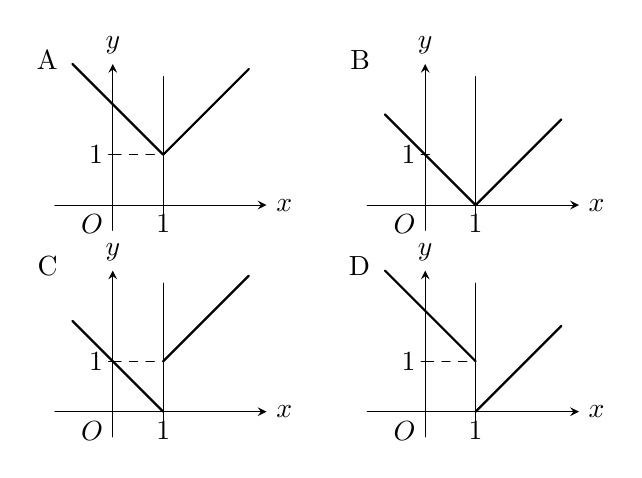
\begin{tikzpicture}[x=0.64cm,y=0.64cm,line cap=round,line join=round,>=stealth]
\begin{scope}
  \draw[->] (-1.15,0)--(3.05,0) node[right] {$x$};
  \draw[->] (0,-0.5)--(0,2.8) node[above] {$y$};
  \draw[thin] (1,-0.35)--(1,2.55);
  \draw[thick] (-0.8,2.8)--(1,1)--(2.7,2.7);
  \draw[dashed] (0,1)--(1,1);
  \draw[thin] (-0.08,1)--(0.08,1) (1,-0.08)--(1,0.08);
  \node[below left] at (0,0) {$O$};
  \node[left] at (0,1) {$1$};
  \node[below] at (1,0) {$1$};
  \node[above left] at (-0.9,2.5) {A};
\end{scope}
\begin{scope}[shift={(6.2,0)}]
  \draw[->] (-1.15,0)--(3.05,0) node[right] {$x$};
  \draw[->] (0,-0.5)--(0,2.8) node[above] {$y$};
  \draw[thin] (1,-0.35)--(1,2.55);
  \draw[thick] (-0.8,1.8)--(1,0)--(2.7,1.7);
  \draw[thin] (-0.08,1)--(0.08,1) (1,-0.08)--(1,0.08);
  \node[below left] at (0,0) {$O$};
  \node[left] at (0,1) {$1$};
  \node[below] at (1,0) {$1$};
  \node[above left] at (-0.9,2.5) {B};
\end{scope}
\begin{scope}[shift={(0,-4.1)}]
  \draw[->] (-1.15,0)--(3.05,0) node[right] {$x$};
  \draw[->] (0,-0.5)--(0,2.8) node[above] {$y$};
  \draw[thin] (1,-0.35)--(1,2.55);
  \draw[thick] (-0.8,1.8)--(1,0);
  \draw[thick] (1,1)--(2.7,2.7);
  \draw[dashed] (0,1)--(1,1);
  \draw[thin] (-0.08,1)--(0.08,1) (1,-0.08)--(1,0.08);
  \node[below left] at (0,0) {$O$};
  \node[left] at (0,1) {$1$};
  \node[below] at (1,0) {$1$};
  \node[above left] at (-0.9,2.5) {C};
\end{scope}
\begin{scope}[shift={(6.2,-4.1)}]
  \draw[->] (-1.15,0)--(3.05,0) node[right] {$x$};
  \draw[->] (0,-0.5)--(0,2.8) node[above] {$y$};
  \draw[thin] (1,-0.35)--(1,2.55);
  \draw[thick] (-0.8,2.8)--(1,1);
  \draw[thick] (1,0)--(2.7,1.7);
  \draw[dashed] (0,1)--(1,1);
  \draw[thin] (-0.08,1)--(0.08,1) (1,-0.08)--(1,0.08);
  \node[below left] at (0,0) {$O$};
  \node[left] at (0,1) {$1$};
  \node[below] at (1,0) {$1$};
  \node[above left] at (-0.9,2.5) {D};
\end{scope}
\end{tikzpicture}
\end{center}
\nopagebreak[4]
\Needspace{4\baselineskip}
\textbf{解析}

$y=|x-1|$ 的图像是顶点为 $(1,0)$、开口向上的 V 形，和原图选项位置对照后对应 B。

\gkanswer{答案：B}

\end{answer}
\begin{answer}
\gksolhead{13}{}

\textbf{题目}：

如果 $a,b,c$ 都是正数，那么在直角坐标系中，方程 $ax+by+c=0$ 所表示的直线不经过（　）。

\begin{gkopts}(4)
\task A．第一象限；
\task B．第二象限；
\task C．第三象限；
\task D．第四象限。
\end{gkopts}

\Needspace{4\baselineskip}
\textbf{解析}

若 $x,y>0$ 且 $a,b,c>0$，则 $ax+by+c>0$，故直线不经过第一象限，选 A。

\gkanswer{答案：A}

\end{answer}
\begin{answer}
\gksolhead{14}{}

\textbf{题目}：

如果椭圆 $4x^2+y^2=k$ 上两点间的最大距离是 $8$，那么 $k=$（　）。

\begin{gkopts}(4)
\task A．$32$；
\task B．$16$；
\task C．$8$；
\task D．$4$。
\end{gkopts}

\Needspace{4\baselineskip}
\textbf{解析}

椭圆半长轴为 $\sqrt{k}$，最大点间距离等于长轴长 $2\sqrt{k}=8$，所以 $k=16$，选 B。

\gkanswer{答案：B}

\end{answer}
\begin{answer}
\gksolhead{15}{}

\textbf{题目}：

如果双曲线经过点 $(6,\sqrt3)$，且它的两条渐近线方程是 $y=\pm\dfrac13x$，那么这双曲线的方程是（　）。

\begin{gkopts}(2)
\task A．$\dfrac{x^2}{36}-\dfrac{y^2}{4}=1$；
\task B．$\dfrac{x^2}{81}-\dfrac{y^2}{9}=1$；
\task C．$\dfrac{x^2}{9}-y^2=1$；
\task D．$\dfrac{x^2}{18}-\dfrac{y^2}{3}=1$。
\end{gkopts}

\Needspace{4\baselineskip}
\textbf{解析}

选项 C 的渐近线斜率为 $\pm1/3$。代入点 $(6,\sqrt3)$ 有 $36/9-3=1$，故该双曲线方程为选项 C。

\gkanswer{答案：C}

\end{answer}
\begin{answer}
\gksolhead{16}{}

\textbf{题目}：

如果 $l$ 和 $n$ 是异面直线，那么与 $l,n$ 都垂直的直线（　）。

\begin{gkopts}(2)
\task A．不一定存在；
\task B．总共只有一条；
\task C．总共可能有一条，也可能有两条；
\task D．必然有无穷多条。
\end{gkopts}

\Needspace{4\baselineskip}
\textbf{解析}

按直线方向夹角的定义，两异面直线的方向不平行；同时垂直于两方向的非零方向由方向向量叉积给出，因此平行于该方向的直线有无穷多条。若题中“垂直”要求直线必须与两异面直线相交，则对应的是唯一公垂线。固定扫描答案表印 D，但仅凭现存题面不能确认原题采用哪种约定，答案保持 U/PENDING。

\gkanswer{答案：U/PENDING}

\end{answer}
\begin{answer}
\gksolhead{17}{}

\textbf{题目}：

侧面都是直角三角形的正三棱锥，当底面边长为 $a$ 时，该三棱锥的全面积是（　）。

\begin{gkopts}(2)
\task A．$\dfrac{3+\sqrt3}{4}a^2$；
\task B．$\dfrac34a^2$；
\task C．$\dfrac{3+3\sqrt3}{2}a^2$；
\task D．$\dfrac{6+\sqrt3}{4}a^2$。
\end{gkopts}

\Needspace{4\baselineskip}
\textbf{解析}

正三棱锥的三个侧面是全等等腰直角三角形，底边 $a$ 为斜边，故每个侧面面积为 $a^2/4$。侧面积为 $3a^2/4$，底面积为 $\sqrt3a^2/4$，全面积为 $(3+\sqrt3)a^2/4$，选 A。

\gkanswer{答案：A}

\end{answer}
\begin{answer}
\gksolhead{18}{}

\textbf{题目}：

如果 $A$ 是第四象限的角，且 $\cos A=\dfrac45$，那么 $\tan\dfrac A2=$（　）。

\begin{gkopts}(2)
\task A．$-3$；
\task B．$\dfrac13$ 或 $-\dfrac13$；
\task C．$\dfrac13$；
\task D．$-\dfrac13$。
\end{gkopts}

\Needspace{4\baselineskip}
\textbf{解析}

\Needspace{5\baselineskip}
$A$ 在第四象限，故 $\sin A=-3/5$。于是
\nopagebreak[4]
\[
\tan\frac A2=\frac{\sin A}{1+\cos A}
=\frac{-3/5}{1+4/5}=-\frac13,
\]
选 D。

\gkanswer{答案：D}

\end{answer}
\begin{answer}
\gksolhead{19}{}

\textbf{题目}：

函数 $y=\sin\left(x+\dfrac\pi5\right)\sin\left(x-\dfrac\pi5\right)$ 的最小正周期是（　）。

\begin{gkopts}(4)
\task A．$4\pi$；
\task B．$2\pi$；
\task C．$\pi$；
\task D．$\dfrac12\pi$。
\end{gkopts}

\Needspace{4\baselineskip}
\textbf{解析}

\Needspace{5\baselineskip}
积化和差得
\nopagebreak[4]
\[
\sin\left(x+\frac\pi5\right)\sin\left(x-\frac\pi5\right)
=\frac{\cos(2\pi/5)-\cos2x}{2}.
\]
其中唯一随 $x$ 变化的项为 $\cos2x$，最小正周期为 $\pi$，选 C。

\gkanswer{答案：C}

\end{answer}
\begin{answer}
\gksolhead{20}{}

\textbf{题目}：

函数 $y=2\sin^2x+2\cos x-3$ 的最大值是（　）。

\begin{gkopts}(4)
\task A．$-1$；
\task B．$-\dfrac12$；
\task C．$\dfrac12$；
\task D．$-5$。
\end{gkopts}

\Needspace{4\baselineskip}
\textbf{解析}

\Needspace{5\baselineskip}
令 $t=\cos x\in[-1,1]$，原式化为
\nopagebreak[4]
\[
2(1-t^2)+2t-3=-2(t-\tfrac12)^2-\frac12.
\]
最大值为 $-1/2$，选 B。

\gkanswer{答案：B}

\end{answer}
\begin{answer}
\gksolhead{21}{}

\textbf{题目}：

如果函数 $f(x)=x^2+2(a-1)x+2$ 在区间 $(-\infty,4]$ 上是减函数，那么实数 $a$ 的取值范围是（　）。

\begin{gkopts}(4)
\task A．$a\le3$；
\task B．$a\ge-3$；
\task C．$a\le5$；
\task D．$a\ge3$。
\end{gkopts}
〔编者注：固定扫描件此处 A 项照录为 $a\le3$；按题设求出的取值范围为 $a\le-3$，与原四个选项均不完全一致。原文照录，待可追溯同版勘误或异本核对。〕

\Needspace{4\baselineskip}
\textbf{解析}

$f'(x)=2(x+a-1)$。在 $(-\infty,4]$ 上递减要求右端点处导数最大值不大于零，即 $f'(4)=2(a+3)\le0$，故数学范围是 $a\le-3$。固定扫描第5页 A 项及答案表照录为 $a\le3$ 与 A；其余选项也不等于完整范围。未推断原题漏印符号，项目答案保持 U/PENDING。

\gkanswer{答案：U/PENDING}

\end{answer}
\begin{answer}
\gksolhead{22}{}

\textbf{题目}：

如果 $x,y$ 是实数，那么“$\cos x=\cos y$”是“$x=y$”的（　）。

\begin{gkopts}(2)
\task A．必要而且充分的条件；
\task B．必要但不充分的条件；
\task C．充分但不必要的条件；
\task D．既不充分也不必要的条件。
\end{gkopts}

\Needspace{4\baselineskip}
\textbf{解析}

若 $\cos x=\cos y$，并不能推出 $x=y$；但 $x=y$ 必推出 $\cos x=\cos y$。所以前者是后者的必要但不充分条件，选 B。

\gkanswer{答案：B}

\end{answer}
\begin{answer}
\gksolhead{23}{}

\textbf{题目}：

满足条件 $|z|=1$ 及 $\left|z+\dfrac12\right|=\left|z-\dfrac32\right|$ 的复数 $z$ 的集合是（　）。

\begin{gkopts}(1)
\task A．$\left\{-\dfrac12+\dfrac{\sqrt3}{2}i,-\dfrac12-\dfrac{\sqrt3}{2}i\right\}$；
\task B．$\left\{\dfrac12+\dfrac12i,\dfrac12-\dfrac12i\right\}$；
\task C．$\left\{\dfrac{\sqrt2}{2}+\dfrac{\sqrt2}{2}i,\dfrac{\sqrt2}{2}-\dfrac{\sqrt2}{2}i\right\}$；
\task D．$\left\{\dfrac12+\dfrac{\sqrt3}{2}i,\dfrac12-\dfrac{\sqrt3}{2}i\right\}$。
\end{gkopts}

\Needspace{4\baselineskip}
\textbf{解析}

$|z+\tfrac12|=|z-\tfrac32|$ 表示点 $z$ 到 $-1/2$ 与 $3/2$ 距离相等，故 $\operatorname{Re}z=1/2$。再与 $|z|=1$ 联立，得 $z=1/2\pm(\sqrt3/2)i$，选 D。

\gkanswer{答案：D}

\end{answer}
\begin{answer}
\gksolhead{24}{}

\textbf{题目}：

如果 $x,y\in\left(0,\dfrac\pi2\right)$，且 $\tan x<\cot y$，那么（　）。

\begin{gkopts}(2)
\task A．$x+y>\dfrac\pi2$；
\task B．$x+y<\dfrac\pi2$；
\task C．$x>y$；
\task D．$x<y$。
\end{gkopts}

\Needspace{4\baselineskip}
\textbf{解析}

$\cot y=\tan(\pi/2-y)$。正切在 $(0,\pi/2)$ 上严格递增，故 $\tan x<\tan(\pi/2-y)$ 等价于 $x<\pi/2-y$，即 $x+y<\pi/2$，选 B。

\gkanswer{答案：B}

\end{answer}
\begin{answer}
\gksolhead{25}{}

\textbf{题目}：

过抛物线 $y^2=4x$ 的焦点作直线交抛物线于 $A(x_1,y_1)$、$B(x_2,y_2)$ 两点。如果 $x_1+x_2=6$，那么 $|AB|=$（　）。

\begin{gkopts}(4)
\task A．$10$；
\task B．$8$；
\task C．$6$；
\task D．$4$。
\end{gkopts}

\Needspace{4\baselineskip}
\textbf{解析}

\Needspace{5\baselineskip}
设非竖直焦点弦所在直线为 $y=t(x-1)$。代入 $y^2=4x$，交点横坐标是方程 $t^2(x-1)^2=4x$ 的两根；两根之和为 $2+4/t^2=6$，所以 $t^2=1$。两根之积为 $1$，故横坐标之差为 $\sqrt{6^2-4}=4\sqrt2$，又 $|y_1-y_2|=|t||x_1-x_2|$，于是
\nopagebreak[4]
\[
|AB|=\sqrt{(x_1-x_2)^2+(y_1-y_2)^2}=8,
\]
选 B。竖直焦点弦 $x=1$ 的横坐标和为 $2$，不符合条件。

\gkanswer{答案：B}

\end{answer}
\begin{answer}
\gksolheadwithlabel{26}{一}{原卷：一}

\textbf{题目}：

（本题满分15分）

本题共有5小题，每小题都有用横线表示的空位，请把你认为合适的内容写在横线上方的空位里，每个小题满分3分。

（1） $\mathrm{tg}\,315^\circ-\mathrm{tg}(-300^\circ)+\mathrm{ctg}(-330^\circ)$ 的值是\gkblank{}。

（2） 函数 $y=\dfrac1{3x+1}$ 的反函数是\gkblank{}。

（3） 过圆 $x^2+y^2=12$ 上的点 $M(3,\sqrt3)$ 作圆的切线，这切线的方程是\gkblank{}。

（4） $\displaystyle\lim_{n\to\infty}\left(\dfrac1{n^2+1}+\dfrac2{n^2+1}+\cdots+\dfrac n{n^2+1}\right)$ 的值是\gkblank{}。

（5） 由 $1,2,3,4$ 四个数字组成的没有重复数字的四位数中，比 $1234$ 大的共有\gkblank{}个（用具体数字作答）。

\Needspace{4\baselineskip}
\textbf{解析}

\gksubpart{（1）}

$\tan315^\circ=-1$、$\tan(-300^\circ)=\sqrt3$、$\cot(-330^\circ)=\sqrt3$，所以原式为 $-1$。

\gksubpart{（2）}

由 $y=1/(3x+1)$ 解出 $x=(1-y)/(3y)$。交换自变量和因变量后，反函数为 $y=(1-x)/(3x)$，定义域 $x\ne0$。

\gksubpart{（3）}

圆 $x^2+y^2=12$ 在 $M(3,\sqrt3)$ 处的切线满足 $3x+\sqrt3y=12$。

\gksubpart{（4）}

\nopagebreak[4]
\[
\frac{1+2+\cdots+n}{n^2+1}
=\frac{n(n+1)}{2(n^2+1)}
\longrightarrow\frac12.
\]

\gksubpart{（5）}

由 $1,2,3,4$ 组成的无重复四位数共有 $4!=24$ 个，1234 是唯一不大于它的一个，故比它大的有 23 个。

\gkanswer{答案（1）：$-1$}

\gkanswer{答案（2）：$y=\dfrac{1-x}{3x}$，$x\ne0$}

\gkanswer{答案（3）：$3x+\sqrt3\,y=12$}

\gkanswer{答案（4）：$\dfrac12$}

\gkanswer{答案（5）：$23$}

\end{answer}
\begin{answer}
\gksolheadwithlabel{27}{二}{原卷：二}

\textbf{题目}：

（本题满分13分）

设 $f(x)=a^{x-1}$，其中常数 $a>0$。

（1） 如果 $\{x_n\}$ 是等差数列，求证 $\{f(x_n)\}$ 是等比数列；

\Needspace{5\baselineskip}
（2） 如果 $a=4$，解方程
\nopagebreak[4]
\[
4f(x)+f(-x)-1=0.
\]

\Needspace{4\baselineskip}
\textbf{解析}

\gksubpart{（1）}

\Needspace{5\baselineskip}
设 $\{x_n\}$ 的公差为 $d$，则 $x_n=x_1+(n-1)d$。因此
\nopagebreak[4]
\[
f(x_n)=a^{x_n-1}=a^{x_1-1}(a^d)^{n-1}=f(x_1)(a^d)^{n-1}.
\]
由于 $a>0$，公比 $a^d>0$，故 $\{f(x_n)\}$ 是等比数列。

\gksubpart{（2）}

\Needspace{5\baselineskip}
当 $a=4$ 时，原方程化为
\nopagebreak[4]
\[
4^x+4^{-x-1}-1=0.
\]
\Needspace{5\baselineskip}
令 $u=4^x>0$，则
\nopagebreak[4]
\[
u+\frac1{4u}-1=0\iff (2u-1)^2=0,
\]
故 $u=\frac12$，于是 $x=\log_4\frac12=-\frac12$。

\gkanswer{答案（1）：见解析版}

\gkanswer{答案（2）：$x=-\dfrac12$}

\end{answer}
\begin{answer}
\gksolheadwithlabel{28}{三}{原卷：三}

\textbf{题目}：

（本题满分14分）

如图，在平面 $\beta$ 内有 $\triangle ABC$，在平面 $\beta$ 外有点 $S$，斜线 $SA\perp AC$，$SB\perp BC$，且斜线段 $SA$ 和 $SB$ 在 $\beta$ 内的射影是等长的线段。
\nopagebreak[4]
\begin{center}% 按固定来源第7扫描页可见点线关系重绘；仅作示意，不按比例，也不增加垂直标记。
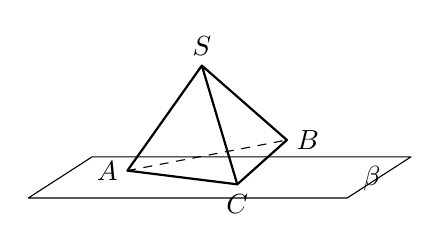
\begin{tikzpicture}[x=0.9cm,y=0.58cm,line cap=round,line join=round]
  \coordinate (P1) at (-2.4,-0.55);
  \coordinate (P2) at (2.1,-0.55);
  \coordinate (P3) at (3.0,0.35);
  \coordinate (P4) at (-1.5,0.35);
  \coordinate (A) at (-1.0,0.05);
  \coordinate (B) at (1.25,0.72);
  \coordinate (C) at (0.55,-0.25);
  \coordinate (S) at (0.05,2.35);
  \draw[thin] (P1)--(P2)--(P3)--(P4)--cycle;
  \node at (2.45,-0.12) {$\beta$};
  \draw[thick] (A)--(C)--(B);
  \draw[dashed] (A)--(B);
  \draw[thick] (S)--(A) (S)--(B) (S)--(C);
  \node[left] at (A) {$A$};
  \node[right] at (B) {$B$};
  \node[below] at (C) {$C$};
  \node[above] at (S) {$S$};
\end{tikzpicture}
\end{center}
\nopagebreak[4]
（1） 求证：$AC=BC$；

（2） 又设点 $S$ 与平面 $\beta$ 的距离为 $3$ 厘米，且 $AC\perp BC$，$AB=4$ 厘米，求线段 $SC$ 的长。

\Needspace{4\baselineskip}
\textbf{解析}

\gksubpart{（1）}

由题设投影等长得 $SA=SB$。两直角三角形 $SAC$、$SBC$ 以公共斜边 $SC$ 和相等直角边全等，故 $AC=BC$。

\gksubpart{（2）}

\Needspace{5\baselineskip}
设 $D$ 为 $S$ 到平面 $\beta$ 的垂足。由三垂线定理的逆定理，$\angle DAC=\angle DBC=90^\circ$。结合 $AC\perp BC$、$AC=BC$，四边形 $ACBD$ 为正方形，故 $CD=AB=4\text{ cm}$。因此
\nopagebreak[4]
\[
SC=\sqrt{SD^2+CD^2}=\sqrt{3^2+4^2}=5\text{ cm}.
\]
\nopagebreak[4]
\begin{center}% 按固定答案扫描页9图4-5-8的可见关系重绘；含平面内投影点D，仅作示意、不按比例。
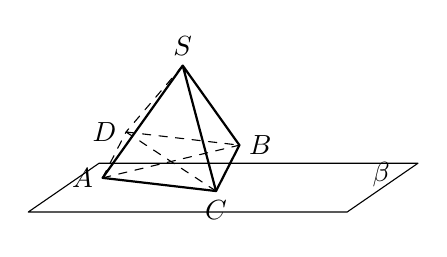
\begin{tikzpicture}[x=0.9cm,y=0.62cm,line cap=round,line join=round]
  \coordinate (P1) at (-2.5,-0.85);
  \coordinate (P2) at (2.0,-0.85);
  \coordinate (P3) at (3.0,0.15);
  \coordinate (P4) at (-1.5,0.15);
  \coordinate (A) at (-1.45,-0.15);
  \coordinate (C) at (0.15,-0.42);
  \coordinate (B) at (0.48,0.52);
  \coordinate (D) at (-1.12,0.79);
  \coordinate (S) at (-0.32,2.15);

  \draw[thin] (P1)--(P2)--(P3)--(P4)--cycle;
  \node at (2.48,-0.08) {$\beta$};

  \draw[thick] (A)--(C)--(B);
  \draw[dashed] (A)--(B);
  \draw[thick] (S)--(A) (S)--(B) (S)--(C);
  \draw[dashed] (S)--(D) (A)--(D) (D)--(B) (C)--(D);

  \node[left] at (A) {$A$};
  \node[below] at (C) {$C$};
  \node[right] at (B) {$B$};
  \node[left] at (D) {$D$};
  \node[above] at (S) {$S$};
\end{tikzpicture}
\end{center}
\nopagebreak[4]
\gkanswer{答案（1）：$AC=BC$}

\gkanswer{答案（2）：$SC=5\text{ cm}$}

\end{answer}
\begin{answer}
\gksolheadwithlabel{29}{四}{原卷：四}

\textbf{题目}：

（本题满分14分）

已知复数 $z=1-2i$，其中 $i$ 是虚数单位。

（1） 求 $\dfrac2{z+i}-\overline{(z+1)}$ 的值，并把该值表示成三角形式；

\Needspace{5\baselineskip}
（2） 求适合不等式
\nopagebreak[4]
\[
\log_{0.5}\frac{|az-i|}{\sqrt{a+1}}\le\frac12
\]
的实数 $a$ 的取值范围。

\Needspace{4\baselineskip}
\textbf{解析}

\gksubpart{（1）}

\nopagebreak[4]
\[
\frac2{z+i}-\overline{(z+1)}
=\frac2{1-i}-(2+2i)
=1+i-(2+2i)
=-1-i.
\]
\Needspace{5\baselineskip}
其模为 $\sqrt2$，可用辐角 $5\pi/4$ 表示，故三角形式为
\nopagebreak[4]
\[
\sqrt2\left(\cos\frac{5\pi}{4}+i\sin\frac{5\pi}{4}\right).
\]

\gksubpart{（2）}

\Needspace{5\baselineskip}
由
\nopagebreak[4]
\[
|az-i|^2=a^2+(2a+1)^2=5a^2+4a+1
\]
且 $\sqrt{a+1}$ 在分母，先有定义域 $a>-1$。二次式 $5a^2+4a+1$ 的判别式为 $-4$，恒正，故定义域上对数真数为正。

\Needspace{5\baselineskip}
因底数 $0.5\in(0,1)$，原不等式等价于
\nopagebreak[4]
\[
\frac{\sqrt{5a^2+4a+1}}{\sqrt{a+1}}\ge\sqrt{\frac12}.
\]
\Needspace{5\baselineskip}
两边非负且分母为正，平方整理得
\nopagebreak[4]
\[
(5a+1)(2a+1)\ge0.
\]
\Needspace{5\baselineskip}
结合 $a>-1$，解集为
\nopagebreak[4]
\[
\left(-1,-\frac12\right]\cup\left[-\frac15,+\infty\right).
\]
扫描页9只载到起始条件，未见此最终解集，故此结果归属于项目独立推导。

\gkanswer{答案（1）：$-1-i=\sqrt2\left(\cos\dfrac{5\pi}{4}+i\sin\dfrac{5\pi}{4}\right)$}

\gkanswer{答案（2）：$a\in\left(-1,-\dfrac12\right]\cup\left[-\dfrac15,+\infty\right)$}

\end{answer}
\begin{answer}
\gksolheadwithlabel{30}{五}{原卷：五}

\textbf{题目}：

（本题满分14分）

\Needspace{5\baselineskip}
设圆 $O$ 的方程为
\nopagebreak[4]
\[
x^2-2x\cos\theta+y^2+2(1+2\sin\theta)y=0,
\qquad 0\le\theta<2\pi.
\]

（1） 当 $\theta$ 变化时，求圆 $O$ 的圆心轨迹的普通方程，并画出轨迹的草图；

\Needspace{5\baselineskip}
（2） 如果又有圆 $S$：
\nopagebreak[4]
\[
x^2+y^2+2y=0,
\]
求 $\theta$ 的值，使得圆 $O$ 与圆 $S$ 的公共弦的长度取最大值（请把满足条件的 $\theta$ 的值都求出来）。

\Needspace{4\baselineskip}
\textbf{解析}

\gksubpart{（1）}

\Needspace{5\baselineskip}
圆心为 $(\cos\theta,-1-2\sin\theta)$。于是
\nopagebreak[4]
\[
x^2+\frac{(y+1)^2}{4}
=\cos^2\theta+\sin^2\theta=1,
\]
即圆心轨迹为 $x^2+(y+1)^2/4=1$。

\gksubpart{（2）}

\Needspace{5\baselineskip}
记 $s=\sin\theta$、$c=\cos\theta$。圆 $O$ 的圆心和半径平方为
\nopagebreak[4]
\[
M=(c,-1-2s),\qquad R^2=c^2+(1+2s)^2.
\]
\Needspace{5\baselineskip}
圆 $S$ 的圆心为 $N=(0,-1)$，半径为 $1$。两圆方程相减，公共弦所在根轴为 $-cx+2sy=0$。圆心 $N$ 到根轴的距离满足
\nopagebreak[4]
\[
\delta^2=\frac{4s^2}{c^2+4s^2}.
\]
\Needspace{5\baselineskip}
因 $c^2+4s^2=1+3s^2$，公共弦长为
\nopagebreak[4]
\[
L=2\sqrt{1-\delta^2}
=\frac{2|c|}{\sqrt{1+3s^2}}\le2.
\]
等号当且仅当 $s=0$，在 $0\le\theta<2\pi$ 中即 $\theta=0$ 或 $\pi$，最大长度为 $2$。

\gkanswer{答案（1）：$x^2+\dfrac{(y+1)^2}{4}=1$}

\gkanswer{答案（2）：$\theta=0$ 或 $\pi$；最大公共弦长为 $2$}

\end{answer}